% ----------------------------------------------------------------------
% Template VERIFICA
% ----------------------------------------------------------------------
% 2020 di d!egofantinelli at jazzmagus@gmail.com
% ----------------------------------------------------------------------

% ---------------------------------- Preambolo
\documentclass[11pt, a4paper]{exam}
\usepackage[T1]{fontenc}
\usepackage{mdframed}
%\usepackage{nicefrac}
%\usepackage[applemac]{inputenc}
%\usepackage[utf8]{inputenc}
\usepackage[italian]{babel}
\usepackage[margin=1.3in]{geometry}
\usepackage{amsmath,amssymb, systeme}
\usepackage{multicol}
\usepackage{graphicx}
\usepackage{tikz}
\usepackage{upquote}
\usepackage{caption}
%\usepackage{fancyhdr}
\usepackage{float}
\usepackage{array}


\renewcommand{\questionshook}{%
    \setlength{\leftmargin}{0pt}%
}
\renewcommand{\choiceshook}{%
    \setlength{\leftmargin}{20pt}%
}

\newenvironment{sistema}% 
{\left\lbrace\begin{array}{@{}l@{}}}% 
{\end{array}\right.} 

% ---------------------------------- Intestazione
\newcommand{\class}{\huge {Verifica di Matematica}}
\newcommand{\term}{1° Quadrimestre}
\newcommand{\examnum}{Verifica numero: 02 | 02}
\newcommand{\examdate}{29 aprile 2021}
\newcommand{\timelimit}{45 minuti}

\CorrectChoiceEmphasis{\color{red}}
\SolutionEmphasis{\color{red} \footnotesize}
\renewcommand{\solutiontitle}{\noindent\textbf{Soluzione:}\par\noindent}
% ---------------------------------- Intestazione

\pagestyle{headandfoot}
\firstpageheader{IIS "G. A. Remondini" - Bassano del Grappa (VI)}{}{\examdate}
\runningheader{\footnotesize VERIFICA di MATEMATICA}{}{Classe 4\string^QA}
\runningheadrule

\firstpagefooter{}{}{pag. \thepage\ di \numpages}
\runningfooter{}{}{pag. \thepage\ di \numpages}
\runningfootrule

% ---------------------------------- Punteggi
\pointpoints{punto}{\em punti}
\pointformat{[{\footnotesize \thepoints}]}
\bonuspointpoints{punto bonus}{\em punti bonus}
\bonuspointformat{[{\footnotesize \thepoints}]}
\pointsinrightmargin
\setlength{\rightpointsmargin}{.2cm}
\chqword{Esercizio}
\chpword{Punti}
\chbpword{Punti Bonus}
\chsword{Punteggio}
\chtword{Totale}


%\printanswers

\begin{document}

% ---------------------------------- Title Page
\begin{center}
\rule[2ex]{\textwidth}{0.5pt}\\
{\huge{\bf \class}}\\[12pt]
%{\huge -\, \term \, - }\\[8pt]
{\huge -\, \examnum \, - }\\[8pt]
\rule[2ex]{\textwidth}{0.5pt}\\
\end{center}
\vspace{3cm}
\vspace{3cm}
\begin{tabular*}{\textwidth}{l @{\extracolsep{\fill}} r @{\extracolsep{6pt}} l}
\textbf{} & \textbf{Cognome e Nome:} & \makebox[2.5in]{\hrulefill}\\
\textbf{} &&\\
\textbf{} & \textbf{Classe:} & \makebox[2.5in]{\Large{\bf 4 \string^ QA}}\\
\textbf{} &&\\
\textbf{} & Tempo a disposizione: & \makebox[2.5in]{\timelimit}
\end{tabular*}\\[3cm]

\vspace{3cm}
% ---------------------------------- Avvertenze

\noindent
%\rule[2ex]{\textwidth}{0.2pt}
\textbf{Avvertenze}:
\begin{itemize}
	\item La presente Verifica di Recupero - che viene somministrata in modalità IN PRESENZA - contiene \numquestions \; quesiti, per un totale di \numpoints \;punti;
	\item Per gli eventuali studenti che dovessero svolgere la prova in DDI, la webcam dovrà  rimanere accesa per tutto il tempo della verifica (\timelimit), salvo impossibilità concrete di connessione; il microfono resterà spento e verrà acceso soltanto per chiarimenti e domande, che saranno consentite negli ultimi 20 min di prova.
	\item E' vietato l'utilizzo di calcolatrici scientifiche, smartphone, tablet e altri dispositivi digitali, nonché la consultazione di testi, appunti e siti web.

\end{itemize}
%\rule[2ex]{\textwidth}{0.2pt}
\vfill
\newpage

% ===================================== Esercizi

%\printanswers

\begin{questions}

% ------------------------------------- Esercizio 1
\addpoints
\question[6]
Determina le soluzioni della seguente disequazione frazionaria di secondo grado:\\

\(\dfrac{x^2 - 9}{x^2 - 6x + 5} > 1\)

%\begin{parts}
%\part[5]
%\(\dfrac{4}{3}x^2 - \dfrac{1}{4} = 0\)\\
%\fillwithlines{0.5in}
{\footnotesize
\begin{solution}
	\( \left[\; S = \left\{ \forall x \in \mathbb{R}: 1 < x < \dfrac{7}{3} \, \vee \, x > 5 \right\} \; \right] \) 
\end{solution}
}
%\vspace{.75cm}
%
%\part[5]
%\(x^2 + 8x + 12\)\\
%\fillwithlines{0.75in}
%{\footnotesize
%\begin{solution}
%	\(x_1 = -2; \, x_2 = -6 \)
%\end{solution}
%}
%\end{parts}
%
%%{\footnotesize
%%\begin{solution}
%%	\(x_1 = -2; \, x_2 = -6 \)
%%\end{solution}
\vspace{.5cm}

% ------------------------------------- Esercizio 2

\addpoints
\question [6]
Dopo averla ricondotta alla {\em forma normale}, determina le soluzioni della seguente disequazione frazionaria di secondo grado:\\
{\footnotesize
{\em suggerimento:} Una disequazione fratta è in forma normale quando al primo membro della disequazione vi è un'unica frazione e al secondo termine \(0\)
}\\

\(\dfrac{x - 2}{x} + \dfrac{2x - 3}{x - 1} \ge \dfrac{1}{x - x^2}\)

%\fillwithlines{0.75in}

{\footnotesize
\begin{solution}
	\( \left[\; S = \left\{ \forall x \in \mathbb{R}: x < 0 \, \vee \, x > 1 \right\} \; \right] \) 
\end{solution}
\vspace{.5cm}
}
%\pagebreak
% ------------------------------------- Esercizio 3
\addpoints
\question [8] Risolvi il seguente sistema di disequazioni frazionarie di secondo grado: \\
%\begin{equation*}
%	\systeme{
%		 \dfrac{3x-x}{x^2 -1} \ge 0,
%		 \dfrac{(2x - 1)(2x + 1)}{x^2 - 2x + 1} \le 0
%		}
%\end{equation*}

%

\syslineskipcoeff{2,8}
\systeme{\dfrac{x - 3}{2x^2 + 3} \leq 0,
\dfrac{x^2 - x - 2}{x} > 0}
%
%\left\{ \begin{array}{ll}
%\dfrac{3x-x}{x^2 -1} \ge 0 \\[20pt]
%\dfrac{(2x - 1)(2x + 1)}{x^2 - 2x + 1} \le 0
%\end{array}

%\( 
%\begin{sistema} 
%\dfrac{3x-x}{x^2 -1} \ge 0 \\[20pt]
%\dfrac{(2x - 1)(2x + 1)}{x^2 - 2x + 1} \le 0
%\end{sistema} 
%\)

%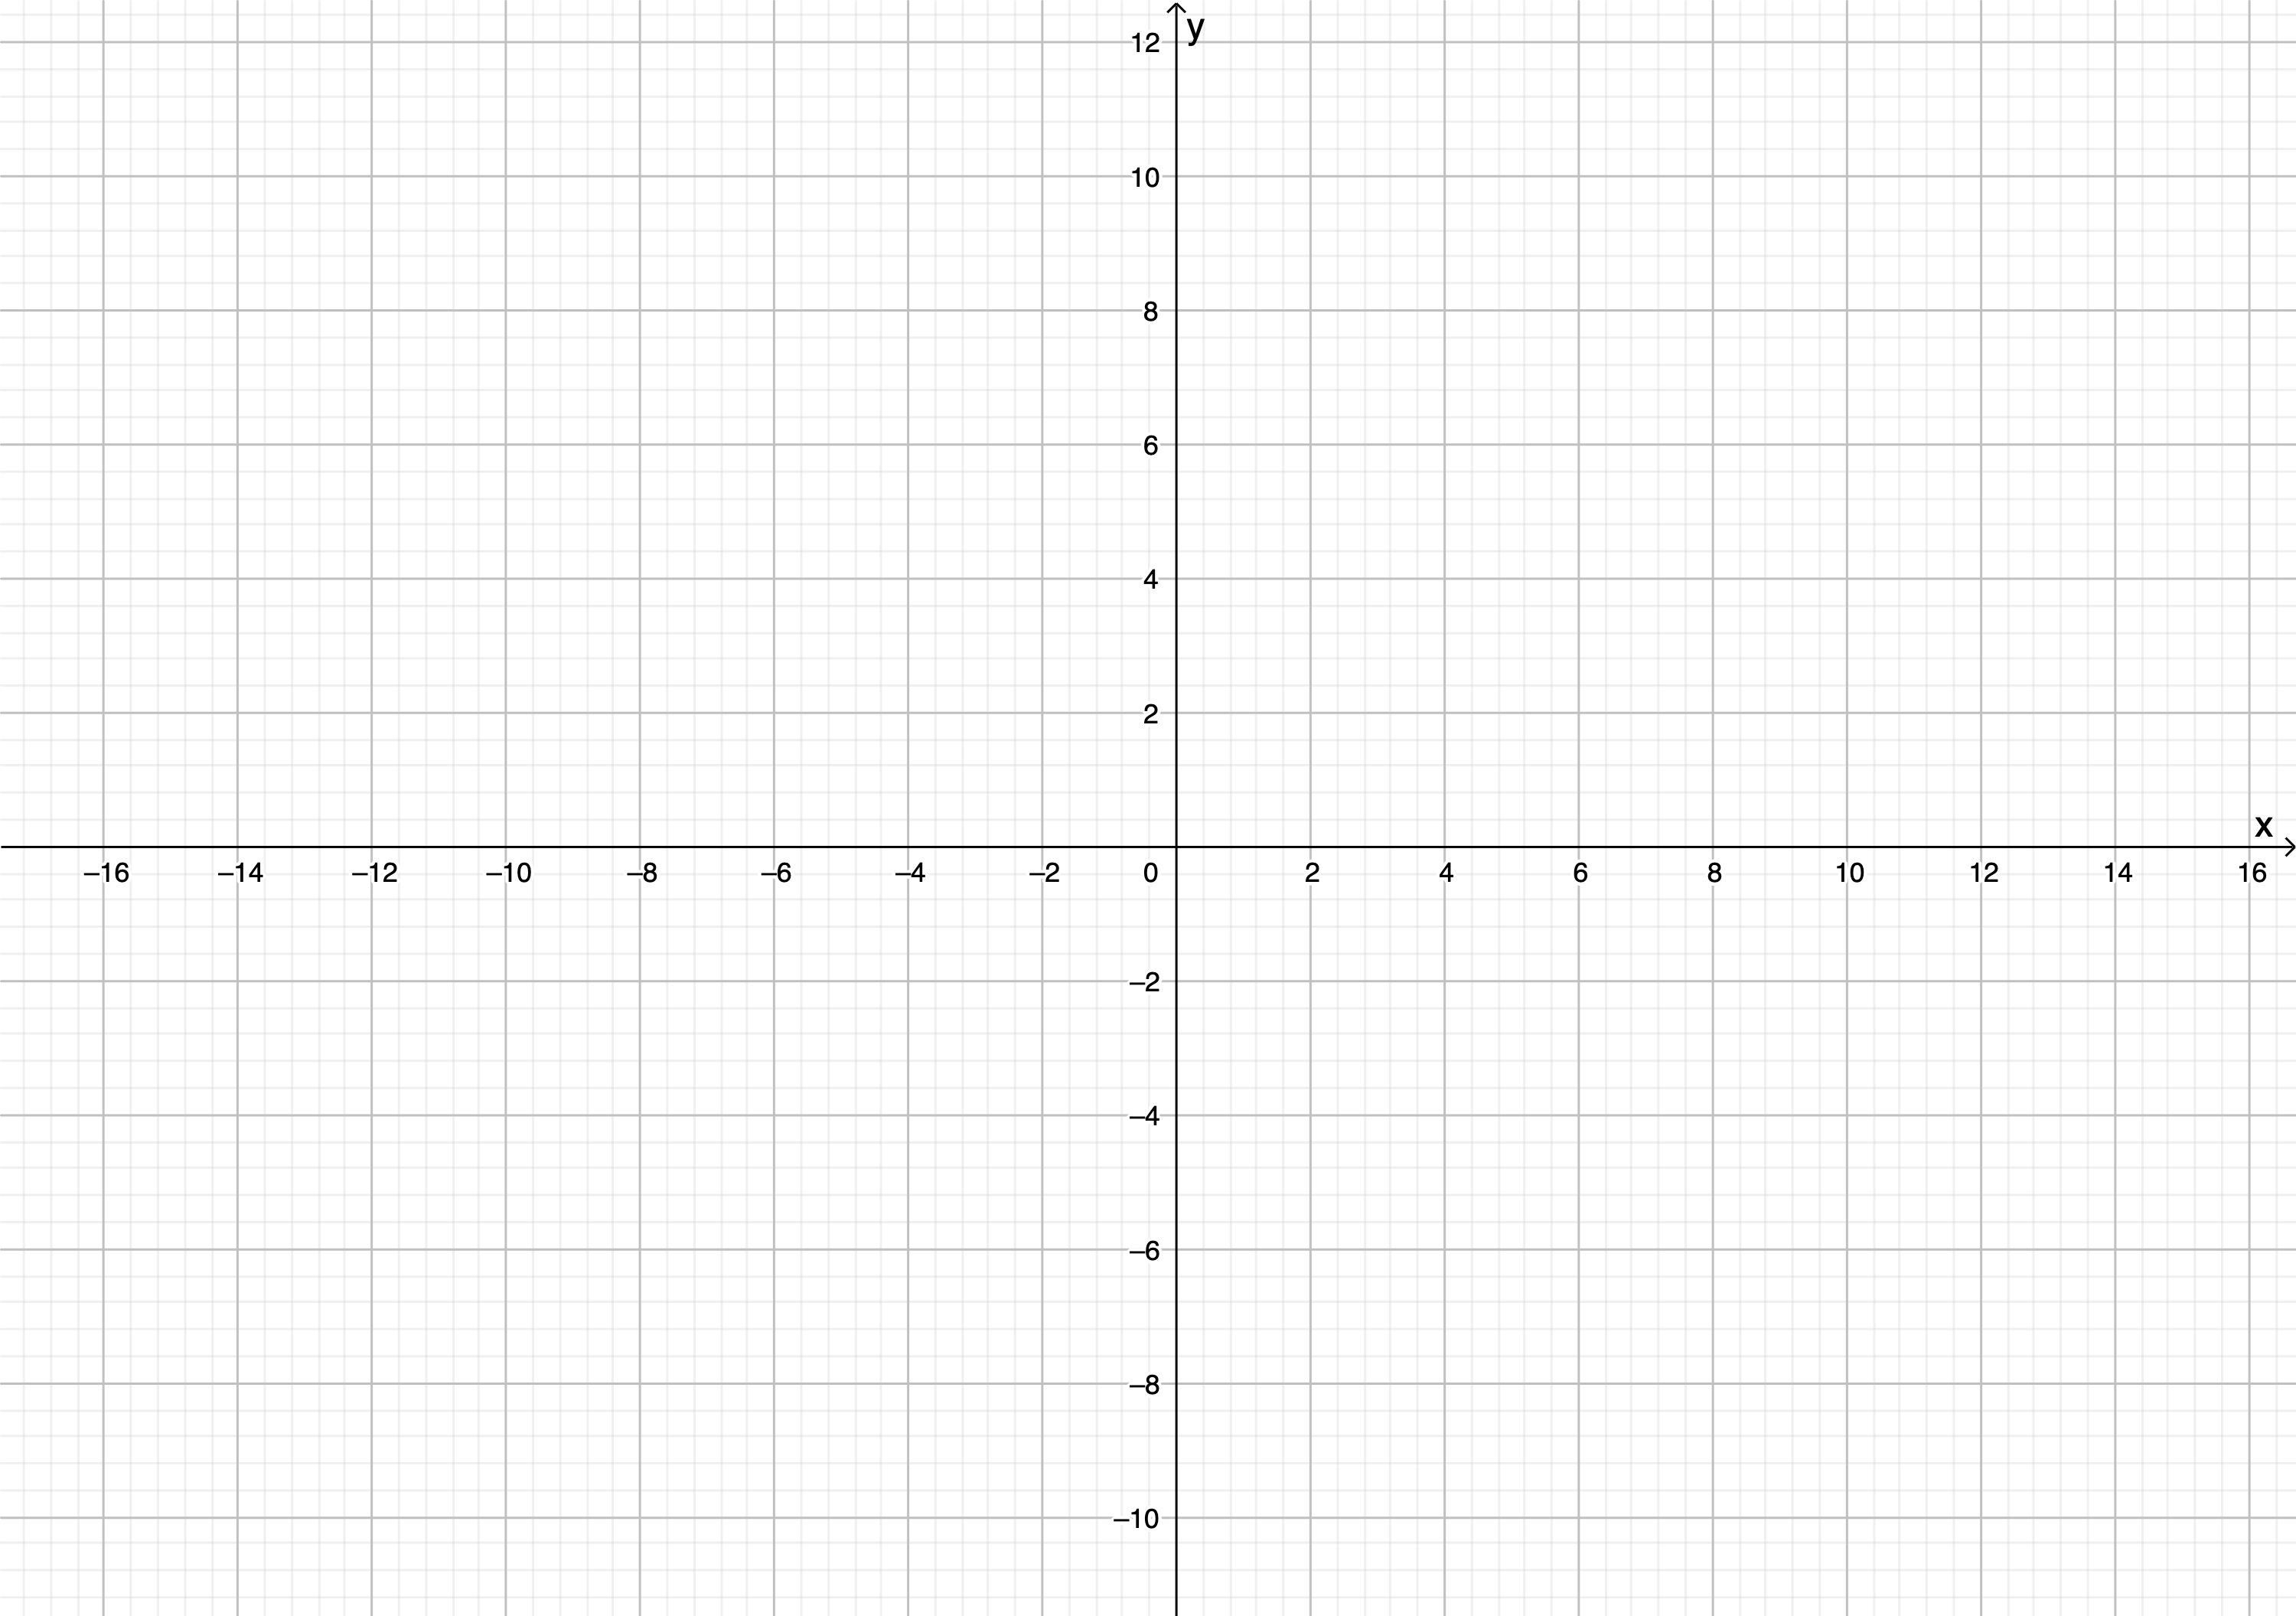
\includegraphics[width=\textwidth]{grafico_empty}
%%\fillwithlines{1in}
%\pagebreak
%% ------------------------------------- Esercizio 4
%\addpoints
%\question [6]
%Quello in figura Ú il grafico di una determinata funzione di secondo grado del tipo \(y = ax^2 + bx + c\);\\
%Ricostruisci l'equazione della funzione aiutandoti con i punti evidenziati:\\
%\vspace{8pt}
%
%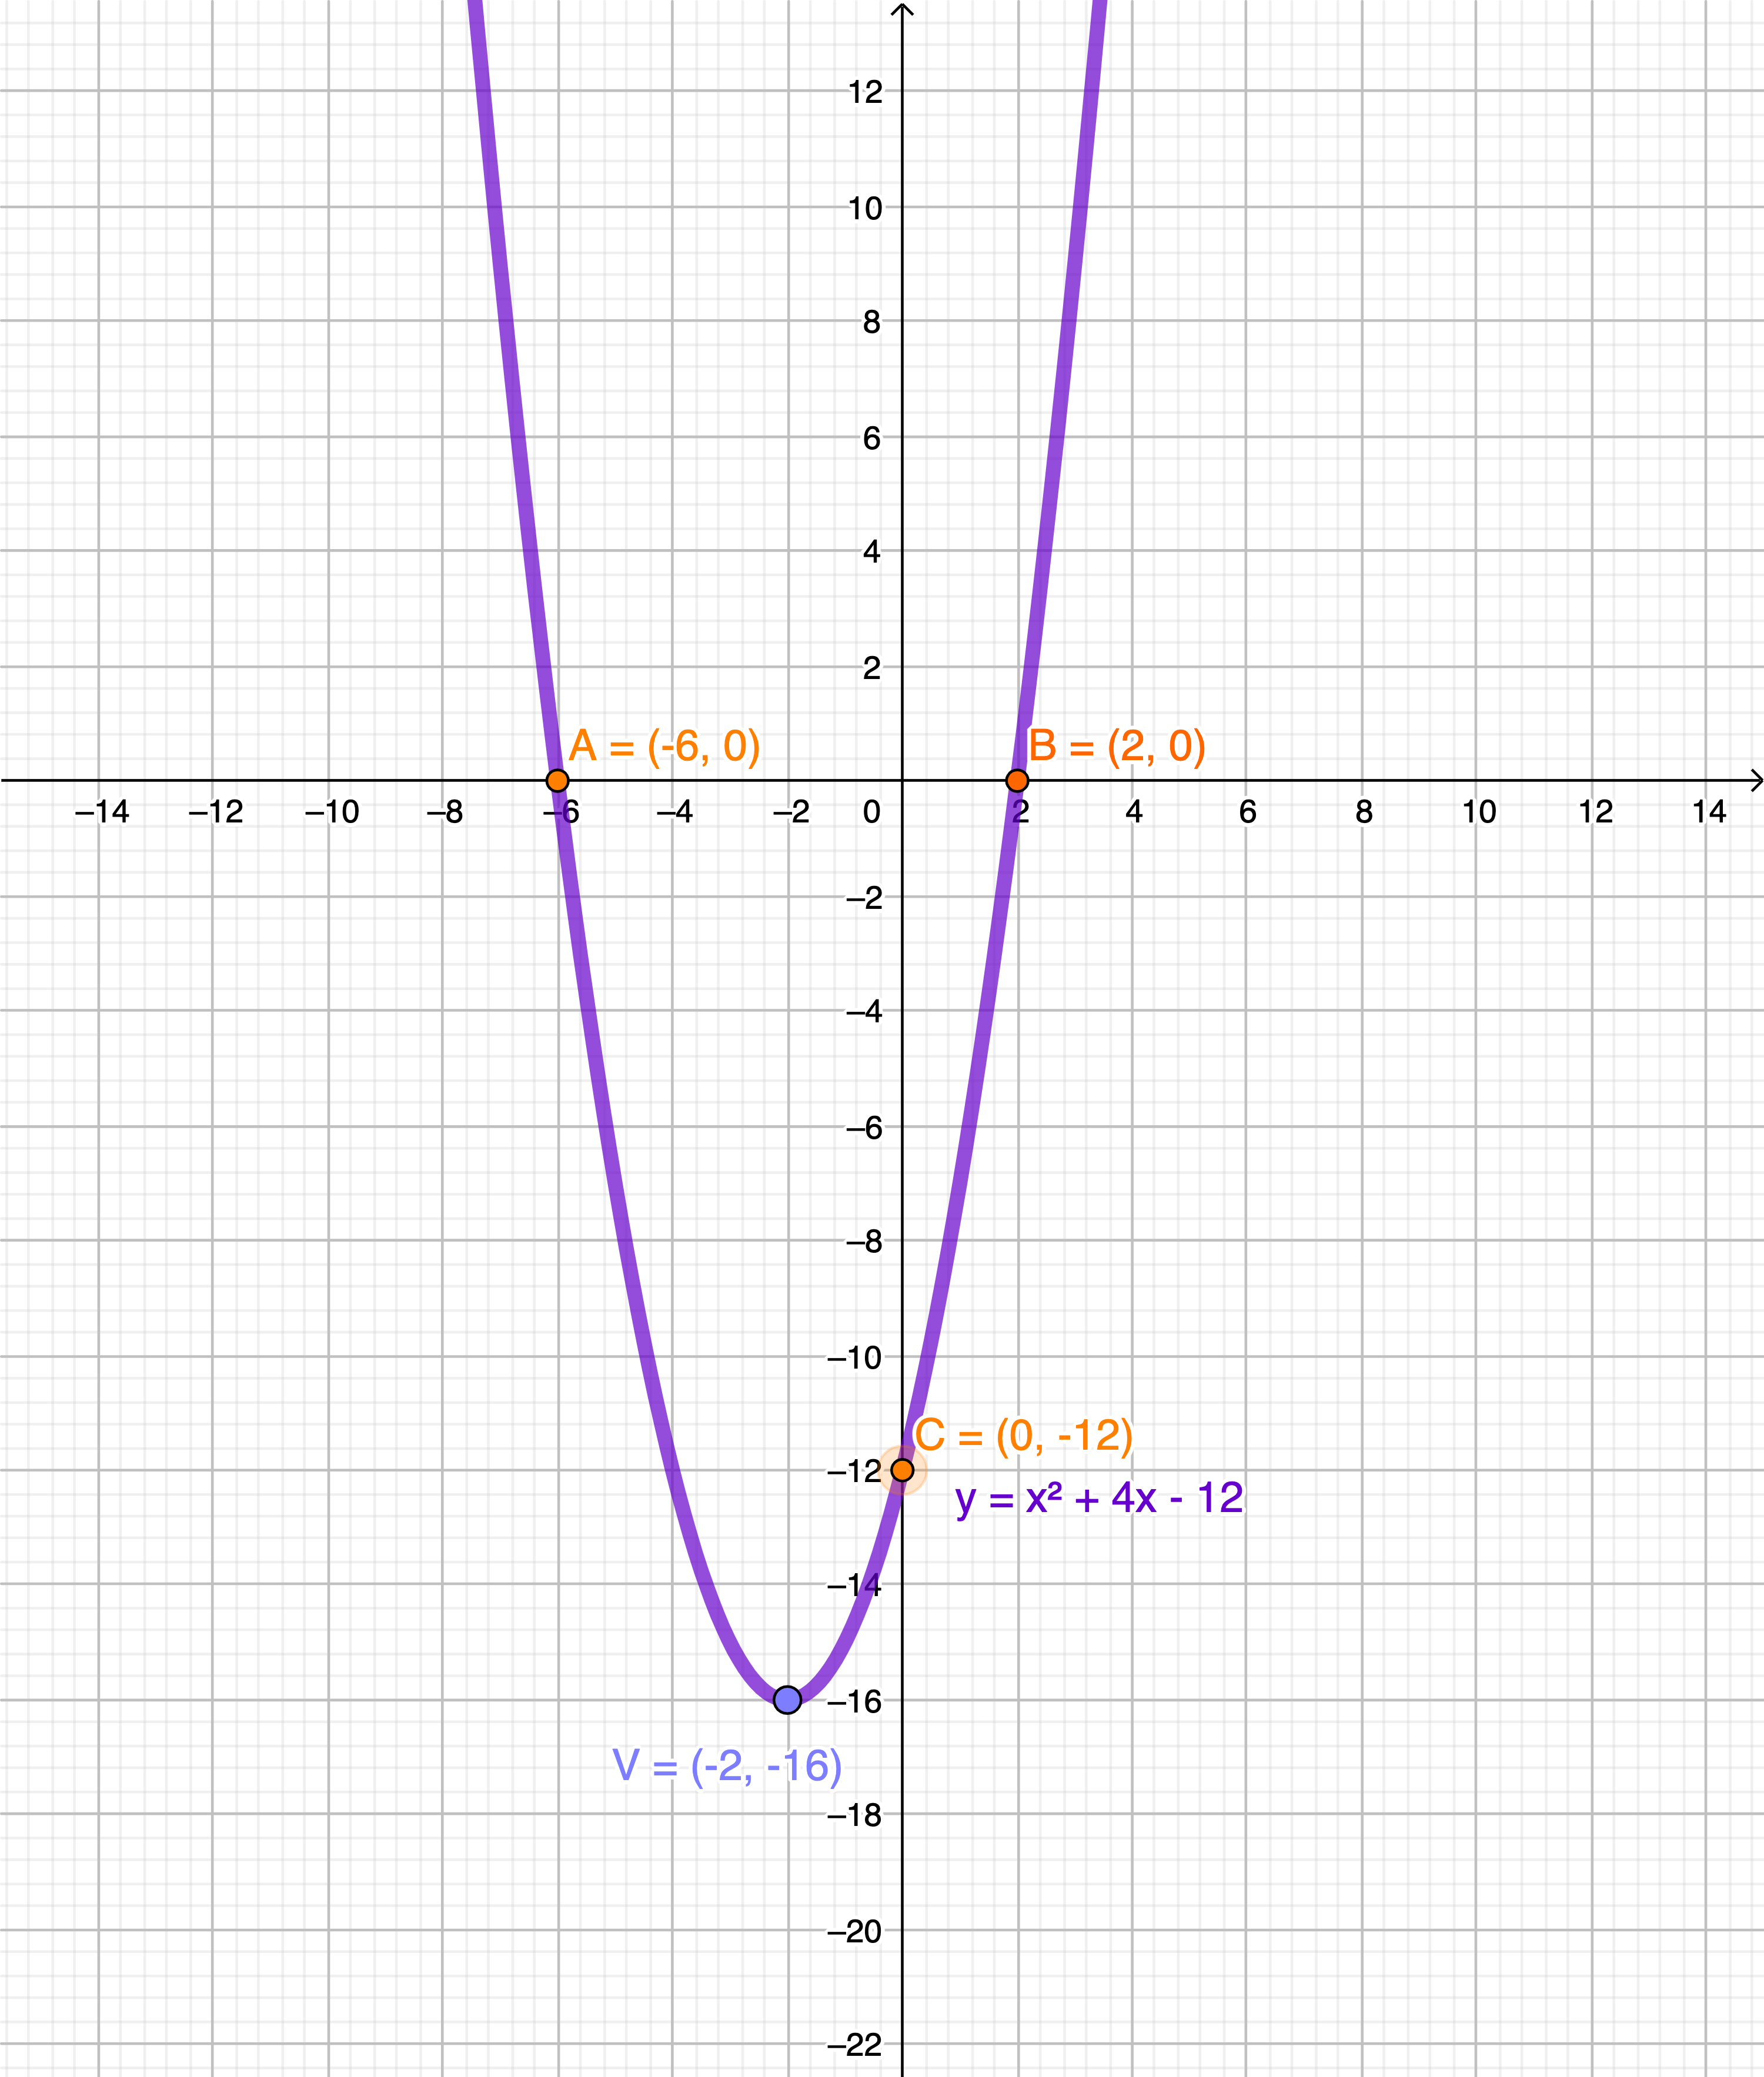
\includegraphics[width=\textwidth]{graph_es3}
%
%\fillwithlines{1in}

{\footnotesize
\begin{solution}	
	\( \left[\; S = \left\{ \forall x \in \mathbb{R}: -1 < x < 0 \vee 2 < x \le 3 \right\} \; \right] \) 
\end{solution}
}

\begin{proof}
To prove it by contradiction try and assume that the statement is false,
proceed from there and at some point you will arrive to a contradiction.
\end{proof}
\end{questions}
\vfill
\rule[2ex]{\textwidth}{1pt}\\
%\pagebreak
\begin{center}
{\bf Tabella dei punteggi}
\vspace{10pt}

\combinedgradetable[h][questions]
\end{center}
\vspace{4pt}
\footnotesize La sufficienza è fissata a 12 punti, ma potrà subire delle modifiche in fase di correzione, al fine di garantire la validità della prova anche nel caso in cui si riscontrino prestazioni della classe sensibilmente lontane dalla media-classe stimata.

\end{document}
